\section{Results}
\label{sec:results}

\todo{Add more results (matter of running more experiments, mostly)}

\subsection{Multi-model Translations}
Figure~\ref{fig:accuracy_nlwiki400_enwiki400_lowercase} shows the accuracy of the multi-model translations.

\begin{figure}[ht!]
  \centering 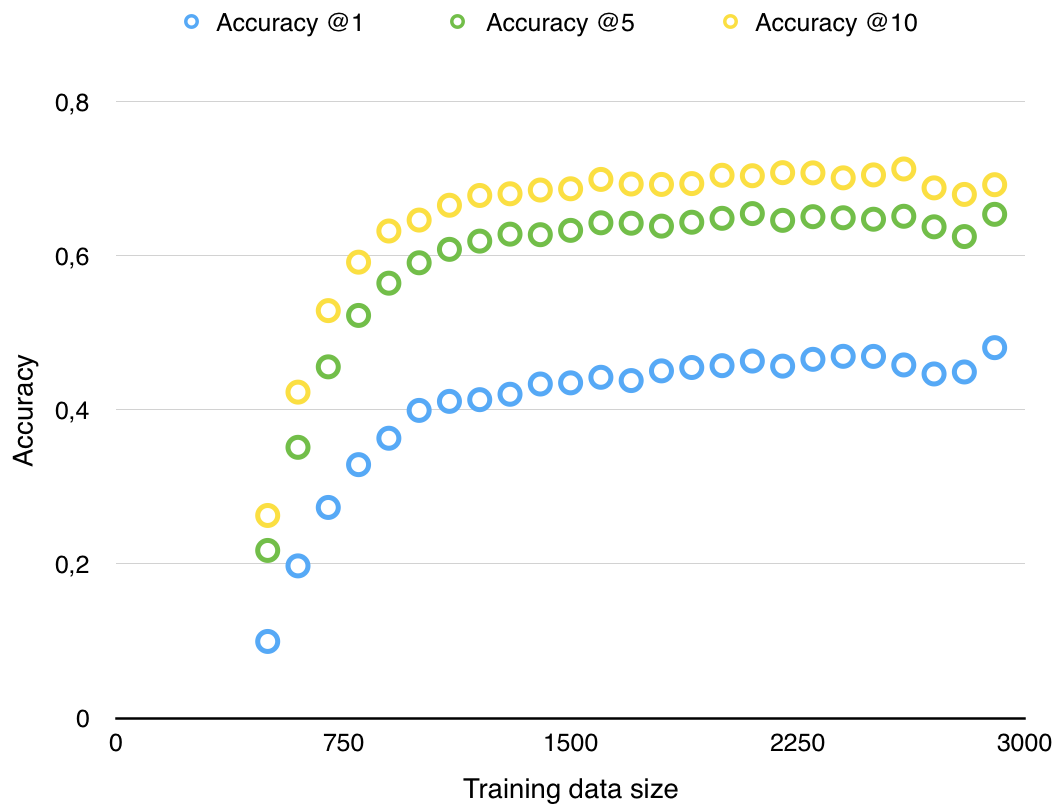
\includegraphics[width=\linewidth]{images/accuracy_nlwiki400_enwiki400_lowercase}
  \caption{Accuracy for different sizes of training dataset for translation matrix, language models trained on Wikipedia at 400 dimensions.}
  \label{fig:accuracy_nlwiki400_enwiki400_lowercase}
\end{figure}

\begin{figure}[ht!]
  % \centering \includegraphics[width=\linewidth]{images/accuracy_nlwiki100_enwiki100_lowercase}
  \caption{Accuracy for different sizes of training dataset for translation matrix, language models trained on Wikipedia at 100 dimensions.}
  \label{fig:accuracy_nlwiki100_enwiki100_lowercase}
\end{figure}

\subsection{Single-model Translations}
\subsubsection{Using Relations}

\subsubsection{Using Translation Matrix}